\documentclass{standalone}
\usepackage{pgfplots}
\usetikzlibrary{shapes.geometric, intersections}
\pgfplotsset{compat=1.7}

\begin{document}
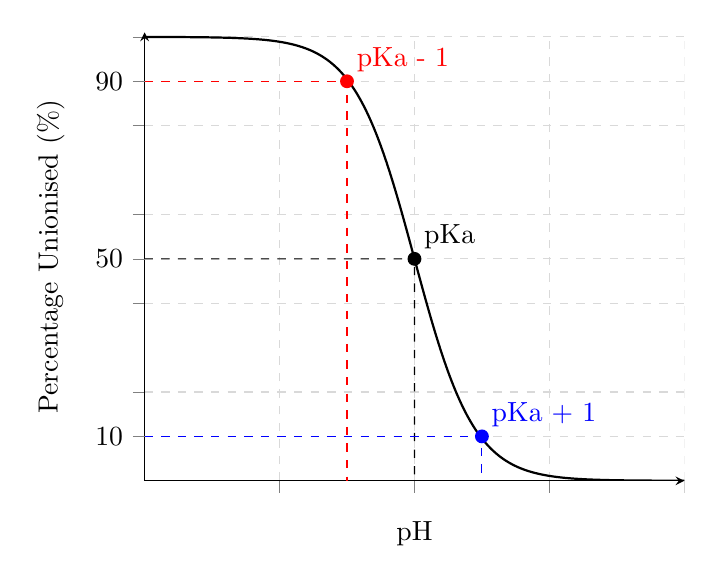
\begin{tikzpicture}

    \begin{axis}[
        axis x line=middle,
        axis y line=middle,
        x tick label style={/pgf/number format/fixed,
                            /pgf/number format/fixed zerofill,
                            /pgf/number format/precision=1},
        y tick label style={/pgf/number format/fixed,
                            /pgf/number format/fixed zerofill,
                            /pgf/number format/precision=0},
        grid = major,
        grid style={dashed, gray!30},
        xmin=0,     % start the diagram at this x-coordinate
        xmax= 0.4,    % end   the diagram at this x-coordinate
        ymin= 0,     % start the diagram at this y-coordinate
        ymax= 101,   % end   the diagram at this y-coordinate
        %axis background/.style={fill=white},
    	  x label style={at={(axis description cs:0.5,-0.1)},anchor=north},
	  y label style={at={(axis description cs:-0.1,.5)},rotate=90,anchor=south},
	  xticklabels={},
	 yticklabels={},
	extra y ticks={10,50,90},
	extra y tick labels = {10,50,90},
	 ylabel near ticks,
	xlabel near ticks,
        xlabel=pH,
        ylabel=Percentage Unionised (\%),
        tick align=outside,
        enlargelimits=false]
	\coordinate (o) at (0,0);
      \addplot[domain=0:0.4, black, thick,samples=500] {100*(1-(1/(1+exp(-45*(x-0.2)))))} node[circle,fill=black,inner sep=0pt,minimum size=5pt,pos=0.5](node1){};

	\draw[black, thin, dashed] (axis cs: 0,50) -- (node1) node[above right]{pKa} -- (node1 |- o) ;


	\draw[blue, thin, dashed]  (axis cs: 0,10) -- (axis cs: 0.25,10) node[circle,fill=blue, thin, dashed,inner sep=0pt,minimum size=5pt]{} node[above right]{pKa + 1} -- (axis cs: 0.25,0);
	\draw[red, thin, dashed]  (axis cs: 0,90) --  (axis cs: 0.15, 90) node[circle,fill=red, thin, dashed,inner sep=0pt,minimum size=5pt]{} node[above right]{pKa - 1} -- (axis cs: 0.15, 0);

\end{axis}

\end{tikzpicture} 
\end{document}